\chapter{Internet of Things: Technologies and Architectures}
\label{ch:iot_tech_arch}
\lhead{Chapter 2. Internet of things: Technologies and Architectures}

The term ``\textit{Internet of Things}"(IoT) was first used in a presentation of Kevin Ashton when presenting his work in The Auto-ID Labs~\footnote{https://autoidlabs.org/}. 
Since then, this paradigm has tremendously gained attention in the scenarios of modern embedded technology, communication technology and information technology.
The IoT was, basically, to refer to an ecosystem of interconnected physical objects that are accessible through the Internet.
As technology evolved its definition has changed, and has been more inclusive covering wide range of applications~\citep{Atzori:2017}. 


Although many definitions of the IoT have been stated by different researchers, business alliances and standardisation bodies~\citep{Minerva:2015}, the main idea of the IoT is the same.
The main goal of the IoT is the integration of physical world with the virtual world that enables a ubiquitous system of sense information.
This integration is being created by enabling physical objects to perceive their surrounding environment, to connect and exchange data among each other and to communicate with people.
As a result, people will be able to monitor and interact with the physical environment remotely from the computer-based systems.
On the other hand, physical objects will be able to derive an understanding of their context, to cooperate with each other, to adaptively interact to changes of their context and thus intelligently assist people.


IoT requires the integration of several technologies.
Embedded technology enables sensors and actuators to be quipped on physical objects; thus they are able to perceive their context and react adaptively to the context.
Communication technology provides networking capabilities; hence, IoT objects can communicate with each other to exchange data an context.
Internet access and user interfaces allows interaction with or provides assistance to people from anywhere and at anytime.
Moreover, semantic, machine intelligence technologies may involve to enable context-awareness and autonomous decision making~\citep{Vermesan:2018}. 

This chapter provides the background knowledge of the Internet of Things. In particularly, section~\ref{sec:history_of_iot} introduces the development of the IoT vision. The enabling technologies for the IoT is presented in Section~\ref{sec:technologies_of_iot}. Finally, we discuss the architectures that enable the IoT in Section~\ref{sec:architecture_of_iot}

%====================================================================
\section{History of IoT}
\label{sec:history_of_iot}
\lhead{2.1 History of IoT}
%====================================================================
The IoT has been defined by researchers, business alliances and standardisation bodies from many domains and different perspectives~\citep{Minerva:2015}.
\cite{Atzori:2010} summarised that IoT would result from the convergence of three main visions: \textit{Thing-oriented vision}, \textit{Internet-oriented vision} and \textit{Semantic-oriented vision}.

%[1999]  
The very first vision of the IoT was derived from the Thing-oriented perspective.
The term ``Internet of Things" was first used in the Auto-ID lab's presentation that introduced Radio-Frequency Identification(RFID) technology. 
An RFID system is composed of RFID readers and RFID tags.
A tags has a unique identifier and is attached in a physical object.
The readers listen to the radio signal from tags to identify the appearance of physical objects in the surrounding area. 
Such RFID systems would allow physical objects to be mapped into the virtual world using RFID readers and RFID tags.
In this early stage, ``Things" simply referred to RFID tags and the IoT was a system of physical objects that were traceable via RFIDs. 
The Unique/Universal/Ubiquitous Identifier(uID)~\citep{Sakamura:2006} and the Electronic Product Code(EPC)~\citep{Armenio:2007} were the following projects that supported the worldwide use of the RFID technology.
These projects aimed to create a global standard for RFIDs that would enable the global identification for physical objects.

%[2005]
It was argued that the IoT would be built up by combing RFID technology and sensing technology~\citep{ITU:2005}.
The RFID tags could respond to the location, label and status of the tagged physical objects.
Sensors could be embedded in the physical objects to provide information about the environment surrounding the objects. 
The integration of the two technologies would enable the fuller understanding on the context of the physical objects.
Wireless sensors and RFID tags attached on moving objects would provide better status of the objects, i.e, their location and temperature, movements, etc.
The IoT vision became wider vision than the idea of a global system of RFID tagged objects, thing's intelligence was considered~\citep{Sterling:2005}. 

%[2006-2009]
According to~\cite{Presser:2009}, the IoT could be more than just a global EPC system of RFID tagged objects.
Devices, networks, services would be soon also viewed as components of the IoT.
However, RFID technology would still be the forefront of the enabling technologies of the IoT.
Together with RFID, the atomic technologies of the IoT would be Near Field Communication(NFC), Wireless Sensor and Actuator Networks(SWAN).
Wireless Identification and Sensing Platforms(WISP) was the project that aimed to create IoT platform based on these technologies~\citep{Buettner:2008}.

%[2014]
More recently, the focus on ``Things" has gone beyond the RFIDs, and the intelligence of IoT ``Things" has been the recent interest~\citep{Sundmaeker:2010}.
The ``Things" mean the ~\textit{Smart Items} which are not only equipped with usual sensors, actuators, wireless communication and elaboration capabilities, but also with new smart and adaptive potentials.
Autonomous and proactive behaviours, context awareness, collaborative communications are just some of these now potentials~\citep{Atzori:2014}.

%[internet-oriented 2005 - 2010]
According to~\cite{Atzori:2010}, the IoT vision that everything would be connected was derived from the \textit{Internet-oriented} perspective.
In 2005, the \textit{International Telecommunication Union} (ITU)  phrased the IoT vision as ``from anytime, anyplace connectivity for anyone, we will now have connectivity for anything". They also stated that the IoT would be ``a global infrastructure for the information society, enabling advanced services by interconnecting (physical and virtual) things based on existing and evolving interoperable information and communication technologies."~\citep{ITU:2005}.


The researches on the Internet-oriented vision attempted to extend the ``Internet of computers" to the ``Internet for everyday objects"~\citep{Mattern:2010}.
For bringing the Internet into a physical infrastructure, the Internet $\emptyset$~\citep{Gershenfeld:2006} simplified the Internet Protocol(IP) to adapt to any object.
Internet Protocol for Smart Objects(IPSO)~\citep{Dunkels:2008} proposed 6LoWPAN protocol for the connectivity on the devices that have limited processing capabilities.
IPv6 could provide larger IP space for the huge number of physical objects and 6LoWPAN allowed transmitting IPv6 packets over low power wireless IEEE 802.15.4 links.

From the Internet-oriented perspective, the IoT would be seen as an integrated part of the ``Future Internet", people and thing would be connected ``Anytime, Anyplace, with Anything and Anyone, ideally using Any path/network and Any service"~\citep{Sundmaeker:2010}.
In this context, ``thing" can be a real/physical entity or digital/virtual entity.
IoT would be an integrated information network of physical and virtual ``thing" that have identities, physical attributes and virtual personalities.  
Research on SOA(service oriented architecture), Web started to pay attention the adoptions for physical ``things" thus enabling such integration~\citep{De:2011, De:2012,Guinard:2009}. 
The idea ''sensing as service" was one of the efforts for enabling the accesses of sensory data through standard service technologies~\citep{Zaslavsky:2013,Perera:2014a}. 
The ``Web of things" was created based on the idea that a ``things" could form a new Web, and Web standards could be reuse to connect and integrate into the Web of physical things~\citep{Christophe:2011}.

Also, it was argued that the IoT only makes its value when the data of the physical world could be collected, analysed and transformed into useful knowledge~\citep{Vermesan:2011}.
The volume and variety of ``things" would poses challenges of how to store, interconnect, search and organise the information generated by the IoT. 
The ideas that the semantic technologies would play the key role in solving these challenges formed the Semantic-oriented vision of the IoT~\citep{Atzori:2014,Barnaghi:2012}.
IoT devices and IoT data can be efficiently discoverable and searchable by providing them semantic description~\citep{Ioan:2009, Chun:2015,Serena:2017}. 
Adding meaningful description for IoT data would also allow the data to be understandable to machines and software agents, thus facilitating the automated interaction among IoT devices and interoperability among existing IoT platforms~\citep{IERC:2015, Ganzha:2017}. 
Moreover, with semantic annotated data, IoT systems could better understand the context, thus creating smarter services~\citep{Perera:2014b}. 

Recently, the developments of IoT continue towards the transformation of everyday physical objects into ecosystems of information, but with new demands and requirements~\citep{Vermesan:2018}.
Recent data technologies such as data analytics, machine learning and artificial are involving the IoT to enhance the knowledge extraction, automation and decision making. 
Additionally, the new requirements of reducing the latency for IoT application have been addressed in order to provide real-time interactive systems between human and machine.
The development of novel networking technology such as 5G network has been starting to provide faster communication.
The processing power is still increasing to allow the new distributed architectures and solutions for the real-time interactions of human and the IoT.  

\newpage
%=======================================================================================
\section{Enabling Technologies of the IoT}
\label{sec:technologies_of_iot}
\lhead{2.2. Enabling Technologies of the IoT}
%=======================================================================================
 
\begin{figure}[ht!]
    \centering
    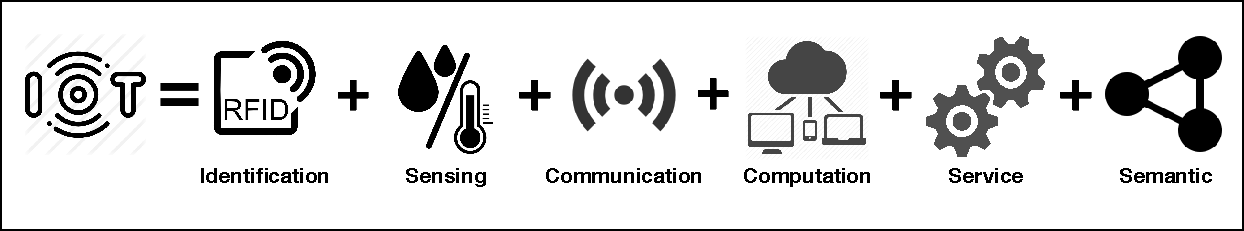
\includegraphics[scale=.75]{Pictures/c2/2-1-IoT-Elements.pdf}
    \caption{The core enabling technologies for the IoT~\citep{Al-Fuqaha:2015}}
    \label{fig:2.2-technologies}
\end{figure}

The previous section discussed the vision and the mission of the IoT. 
The IoT would not be built up from a single technology, but multiple technologies. 
According to ~\cite{Al-Fuqaha:2015}, there have been six core enabling technologies that are required for developing the IoT.
As illustrated in Figure~\ref{fig:2.2-technologies}, the six enabling technologies include: identification technology, sensing technology, communication technology, computation technology, service technology and semantic technology.
In order to provide the better understanding on the IoT, each of IoT technologies is briefly introduced in this section.


\subsection{Identification technologies}
\label{subsec:identification}

The IoT is a system of global interconnected ``things" and IoT applications are typically built based on the integration of these ``things".
In order to ensure the correct integration, the "things" must be uniquely identifiable. 
As the ``things" can be physical entities (e.g. sensors, devices) or virtual entities (e.g. services, computational processes), the technologies for globally identifying of physical and virtual objects are crucial for the development of the IoT.

The identification for physical objects such as computer, mobile devices, networking devices, sensors has already been developed.
The physical objects can be identified by their associated identifier such as a host name, an IP address or URI (Universal Resource Identifier).
The identifiers may contain the additional information of the relationship of physical objects or their locations.
Moreover, the technologies for identifying virtual objects such as services, datastores, web objects, digital documents have also been implemented.
For example, URLs (Universal Resource Locators) has been used for identifying, locating web services, or digital documents can be referenced with DOI(Digital Objects Identifiers).

\begin{table}[ht!]
    \centering
    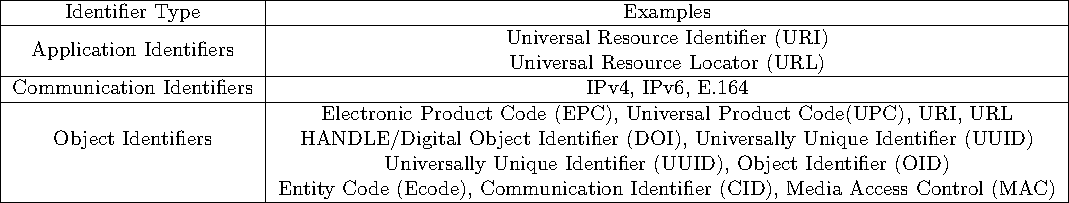
\includegraphics[scale=.85]{Table/2-1-identfication.pdf}
    \caption{Caption}
    \label{tab:IoTIds}
\end{table}

\cite{Presser:2016} reported the available identification methods in the IoT. 
These methods serve different purposes and operate at different layers.
IoT identifiers can be classed into: 
(i) Objects identifiers which are simply used for defining the unique of physical/virtual objects;
(ii) Communication identifiers which are used to uniquely identify connected objects in the context of communications with other objects;
(iii) Application identifiers which are used to identify services, applications. 
The examples of identifiers for the IoT are provided in Table~\ref{tab:IoTIds}

The identification for IoT is composed of three technologies: IoT ID naming, IoT ID addressing and IoT ID discovering~\citep{Presser:2016}.
Naming means assigning labels or attributes to objects or a group of objects to individualise or specify them among larger set of objects.

Addressing is to assigning addresses for connected objects within a communication network.
Addressing also provide the means for mapping of the identifiers at different layers to the communication identifiers.
IoT discovering is the process of locating devices, services or data. 
There are various approaches for the discovery in the IoT, for example, geographic location-based discovery approach~\citep{Dinh:2017}, semantic web-based discovery approach~\citep{Serena:2017}.

---
\nop{
The IoT ID naming technologies have been used including: CID (Communication Identifier), ECODE (Entity Code), HANDLE/DOI
name: OID (Object Identifier) , IPV6, Handle/DOI, BAR CODES and RFID, URIs and UUIDS,
address: DNS (Domain Name Systems), HANDLE
discovery: Resource Discovery in web of things, device abstraction in m2m,

As IoT is a system of interconnected ``things", its applications are typically based on the integration of these ``things".
Similarly to any interactive system, the unique identification of ``thing" is require to ensure the correct integration.
Identification is critically important for any system that requires the interaction between different components. 
The identification of each component in a system is needed to ensure the correct integration of the system.
The IoT could be seen as a global interaction system and its components are users, services, devices and physical objects.
Therefore, ``things" in the IoT must be identified in order to enable such interaction.
    
Due to the continuous increase of the connected devices, providing scalable addressing and identification mechanism is challenging for the IoT. 
The designs of such mechanisms also have to cope to the heterogeneity of the ``things" which could be physical objects or virtual objects. 
Physical objects such as wireless sensors, mobile devices, computers are associated with identifiers such as host names, IP addresses.
Whereas, virtual objects could be identified by the mechanisms, for example, ULRs (Universal Resource Locators) for identifying web services, or DOIs (Digital Objects Identifiers) for referencing digital documents.
The identification for the IoT would be required to address the full range of physical and virtual objects.}




\subsection{Sensor Networks}

%what is sensing
Sensing technologies are the key enablers of the integration of physical world and the virtual world.
Sensors are the electronic devices that can detect events, changes in its environment or measure the quantity of the physical properties.
By converting the signals from physical stimuli into digital form that is readable by machines, sensors allow the IoT understand the environmental characteristics surrounding physical things.

In order to increase the capability of observing the physical world in the IoT, multiple sensors are formed sensor networks.
In the sensors networks, sensors can communicate with each other via wire or wireless connectivity. 
With the better mobility and lower cost, wireless sensors are more attractive for deploying sensor networks~\citep{Sheng:2015}.

%raw data need to be describe

\subsection{Communication}

Communication is the backbone technology of the IoT that connects heterogeneous objects, devices together to provide smart services. 
IoT devices are resource constrained devices, IoT nodes should operate using low power in the presence of lossy and noisy communication links.
This section provides the overview of networking technologies that enable the communication for the IoT.


\subsubsection{Wireless Network Technologies}

%[Low-range]

\textbf{Near Field Communication} is low-range wireless connectivity technology which allows small data to be transmitted over distance of few centimetres. 
Similarly to RFID, NFC transfers data by generating magnetic field and operates over a frequency band of 13.56 MHz.
However, NFC allows both one-way and two-way communications between two devices.
Furthermore, NFC has two operating modes: active and passive.
In active mode, both the sender and the receiver  generating their own fields.
Passive mode is useful for saving energy as only one device generates the field, and the other answers by modulating the existing field.

\textbf{Bluetooth} is the wireless technology that uses short-wavelength UHF radio for exchanging data over short distance.
Compared to NFC, Bluetooth supports broadcasting and provides wider range connectivity with higher frequency and data throughput. 
\textit{Classic Bluetooth} offers enough throughput for data stream application, however, it has several limitations including limited number of nodes in the network.
\textit{Bluetooth Low Energy} or ``\textit{Bluetooth smart}" is advanced over Classic Bluetooth.
It consumes less energy, supports unlimited number of nodes, however, it does not support data streaming and offers lower data rate.
The recent version, \textit{Bluetooth 5.0}, increase the communication range up to 300m and doubles the speed of the low energy connections. 

\textbf{Zigbee} is another low-cost, low-power wireless technology which is based on IEEE 802.15.4 communication protocol.
Compared to Bluetooth or NFC, it offers lower data transferring rate but  much wider communication range.
Depending on power output, outdoors with line-of-sight of Zigbee may range up to 1500m.
Zigbee devices are of there types: Zigbee Coordinator(ZC), Zigbee Router(ZR), Zigbee End Device (ZED).
ZED devices are the simplest devices in Zigbee networks, they just have basic functionalities to communicate with its parent which can be ZC or ZR. 
In a Zigbee network, ZC device is the most capable device whose roles are the root of the network and the bridge to other networks.
Whereas, ZR devices are the intermediate routers for passing data from devices to devices internally. 

\textbf{Z-Wave} is popularised as low-power wireless communication technology for Home Automation Networks.
It covers about 30 meters point-to-point communication, therefor, being widely used in remote applications in smart homes.
Z-wave operates in ISM band around 900MHz and the recent version supports transmission rate up to 200Kbps.

\textbf{Low Power WiFi} is also known as ``WiFi HaLow", which is based on IEEE 802.11ah standard.
The development of WiFi HaLow attempts to extend the range of transmission and to reduce the energy consumption for the WiFi.
Compared to conventional WiFi(IEEE 802.11 b/g/n), the range that HaLow can communicate is doubled.
Wireless sensor networks are the motivated scenarios of HaLow, in which, the devices are energy constrained and require relatively long range connectivity. 

\textbf{Low Power Wide Area Network (LPWAN)}  is a class of the very long range wireless technologies that are suitable for low power application. They can support up to 10 Km distance, however, very low data rate. The technologies in this class include SigFox, LoRaWan and Weightless. 

\textbf{Cellular networks} such as 3G,4G, LTE can provide high-speed connectivity to the Internet for mobile devices. These technologies are based on GSM/UMTS technologies, providing multicasting and broadcasting for fast-travelling devices.
However, they have high power consumption profile.
The under-developing 5G network is expected to be rolled out by 2020 which targets high data rate, reduced latency, energy saving, cost reduction, higher system capacity, and massive device connectivity

\begin{table}[ht!]
    \centering
    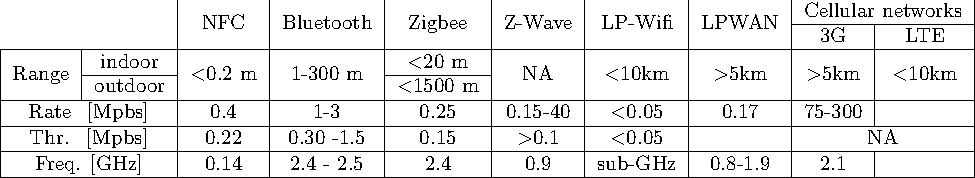
\includegraphics[scale=.95]{Table/2-2-wireless.pdf}
    \caption{Caption}
    \label{tab:my_label}
\end{table}

\subsubsection{Network Protocols}

The full conventional IP suite is very complex and requires a large amount resource on the connecting devices.  
Therefore, the Internet Engineering Task Force(IETF) and IPSO Alliance have been developing alternatively protocols for resource constrained devices in the IoT~\citep{Ishaq:2013, alliance:2011}. 

The IEEE 802.15.4 protocol is designed as a standard for physical and link layers for low-rate wireless personal area networks(PL-WPAN).
To cope with resource constrained environment, it comes with a small frame size, low bandwidth and low transmit power.
Therefore, this protocol can support low power consumption, low data rate, low cost and high message throughput for devices that need a long battery life.

In the Internet layer, IPv6 can provide larger IP addressing space for the large number of IoT devices. 
However, IPv6 was initially developed not thought to be suitable for low-power wireless links.
6LoWPAN which is an acronym of IPv6 over Low-Power Wireless Personal Area Networks provides an adaption layer that allows IPv6 packet to be transmitted over IEEE 802.15.4 links.
To connect with the Internet, 6LoWPAN networks requires a gateway to convert IPv6 and IPv4 as today’s deployed Internet is mostly IPv4. 
The header of IPv6 is lager than the \textit{maximum transmission unit}(MTU) of 802.15.4, 6LoWPAN proposes the following optimisation:
(i) Compressing the header of IPv6 by deleting some of the fields that can be derived from link level and be shared across packets;
(ii)Fragmenting the IPv6 packets into small packets;
(iii) Forwarding to link-layer to support routing and multi-hop delivery.

In the Network layer, the IETF Routing over Low Power and Lossy Networks(ROLL) working group standardised a routing protocol based on IPv6 for resource constrained node called RPL.
RPL was optimised to meet only the minimal routing requirements over lossy links while supporting from simple to complex routing topology.


%[rewrite]
The conventional Internet often uses HTTP application protocol, however, HTTP is not suitable for IoT resourced constrain nodes.
The \textit{IETF Constrained RESTful Environments} (CoRE) working group created \textit{Constrained Application Protocol} (CoAP) that simplifies the HTTP to meet the resource constrained environment of the IoT. 
CoAP also uses REST principles on top of HTTP functionalities, utilises methods such as GET, PUT, POST and DELETE to perform Create, Retrieve, Update and Delete (CRUD) operations.
Therefore, CoAP can be considered as an alternative version of HTTP.
However, to be suitable for resource constrained applications, CoAP is bound UDP rather than TCP.
Unlike HTTP, CoAP uses  EXI (Efficient XML Interchanges) data format, which is space efficient comparing to plain text HTML/XML.
A typical CoAP message can be between 10 to 20 bytes.

\textit{Message Queue Telemetry Transport} (MQTT) is application protocol for messaging developed by IBM.
MQTT is built on top of TCP with a publish/subscribe pattern.
It consists of three components: subscriber, publisher and broker.
The publisher and the subscriber are registered to send/receive data to/from a specific topic.
The broker handles data transmission between publisher and subscriber that are registered to the same topic.
The connection operation uses a routing
mechanism (one-to-one, one-to-many, many-to-many) and enables
MQTT as an optimal connection protocol for the IoT
and M2M.
The initial version of MQTT only operates over TCP which cannot be used with all types of IoT devices, and the topic name 
is represented in text that increases its overhead.
The latter version of MQTT-SN was optimised the earlier version for sensor networks and constraint devices.
It supports UDP mapping and indexing on topic names. 
It is designed for small code footprints and can be implemented in devices with less than 64kb of RAM.

\subsection{IoT hardware and software}

Computational units are the atomic components of the IoT, various hardware platforms and software were developed to run IoT applications. 
Recent advances in the technologies of embedded processor have increased the processing capabilities of IoT devices.
Many devices now can be deployed in network via different communication technologies.
Based on the computational capability, IoT devices can be categorised into two categories~\citep{Hahm:2016}: \textit{low-end}  and \textit{high-end}.
The low-end IoT devices are very constrained in terms of resources including energy, CPU(less than 100MHz) and memory capacity (less than 100 kB).
Popular examples of devices in such category include 
Arduino~\footnote{https://www.arduino.cc/}, 
Zolertia~\footnote{https://zolertia.io/}, 
OpenMote node~\footnote{http://www.openmote.com/}, etc.
The second category consist in high-end IoT devices, which includes single-board computer such as Raspberry Pi~\footnote{https://www.raspberrypi.org/}, 
Beagle Bone board~\footnote{https://beagleboard.org/bone} or 
smartphones.
The high-end devices are more powerful than the low-end devices.
They have enough resources and adequate characteristic to run software based on tradition operating systems such Linux or BSD. 


Furthermore, many IoT software platforms are utilised to provide programming frameworks, programming frameworks, ma-chine-to-machine (M2M) integration, data and device management, security and storage, and protocol translation. 
Several real-time operating systems were specifically developed for the limited resource devices such as low-end IoT devices.
The list of the available of operation systems for IoT can be found in~\citep{Hahm:2016}.
Among of these operating systems, the Contiki~\citep{Biljana:2017}, TinyOS~\citep{Amjad:2016}, LiteOS~\citep{Vanitha:2010} and RiotOS~\citep{Baccelli:2013} have been used widely in many IoT scenarios. 


Moreover, cloud infrastructures are another important computational resources for the IoT~\citep{Botta:2016}.
The cloud computing has been a mature technology and has been considered as an unlimited capabilities storage and processing power.
The IoT also has been integrated with the cloud computing that introducing the \textit{``Cloud of Things"}~\citep{Jiehan:2013} or the ~\textit{``IoT Cloud"}~\citep{Truong:2015}.
These cloud-based systems allow IoT data to be uploaded into cloud where data is processed, and the requesting results are sent back to the IoT devices or IoT applications.
There many cloud platforms and frameworks available to host IoT services such as IBM Bluemix IoT platform~\footnote{https://console.ng.bluemix.net/}, Oracle IoT cloud~\footnote{https://cloud.oracle.com/iot} or Microsoft research Lab of Things~\citep{Brush:2013}.

\subsection{Services}

There four classes of IoT services that are available in many researches references: ~\textit{Identity-related Services}, \textit{Information Aggregation Services}, ~\textit{Collaborative-Aware Services} and ~\textit{Ubiquitous Services}~\citep{Mohammed:2015}.
Identify-related services are the most basic but important services. 
As presented in Section~\ref{ss:identification}, every device that connected to the IoT network has to be identified.
Therefore, every application, service in the IoT requires this type of services to identify the things that are involving. 
Raw sensory data is collected, processed and reported to the to IoT application using Information Aggregation services. 
Collaborative-Aware services are the smart services that can make smart decisions.
These services are often built on top of the Information Aggregation services and able to react accordingly to information provided by the Information Aggregation services.
Ubiquitous services aim to provide Collaborative-Aware services to anyone, from anywhere, at anytime.
The ultimate goal of all IoT applications is to enable the Ubiquitous services.
However, this goal is not easy to achieve, most of the existing applications provide identity related, information aggregation, and collaborative-aware services~\citep{Al-Fuqaha:2015}.
A \textit{smart city}~\citep{Jin:2014, Zanella:2014} which could be seen as an application of ubiquitous services, aims to improve the quality of life in the city by making it easier an more convenient for the residents to find information of interest.

\subsection{Semantic}

%[rewrite]
Semantic in the IoT refers to the ability to extract knowledge smartly by different machines to provide the required services.
Knowledge extraction includes discovering and using resources and modeling information.
Also, it includes recognizing and analyzing data to make sense of the right decision to provide the exact service [62]. 
Thus, semantic represents the brain of the IoT by sending demands to the right resource. 
This requirement is supported by Semantic Web technologies such as the Resource Description Framework (RDF) and the Web Ontology
Language (OWL).
In 2011, the World Wide Web consortium (W3C) adopted the Efficient XML Interchange (EXI) format as a recommendation [63].
EXI is important in the context of the IoT because it is designed to optimize XML applications for resource-constrained environments. 
Furthermore, it reduces bandwidth needs without affecting related resources such as battery life, code size, energy consumed for processing, and memory size. 
EXI converts XML messages to binary to reduce the needed bandwidth and minimize the required storage size.



%=======================================================================================
\section{IoT Architectures}
\label{sec:architecture_of_iot}
\lhead{2.3 IoT Architectures}
%=======================================================================================


In the early stages of research in this areas, three-layer architecture as show in Figure~\ref{fig:2.3-iot-architecture}a was proposed~\citep{Wu:2010,Yang:2011}. 
The IoT could be built up with three layers defined as \textit{perception layer}, \textit{network layer} and \textit{application layers}:

\begin{itemize}[noitemsep,nolistsep]
\item Perception layer: 
This layer is also know as physical layer or sensor layer and is the bottom of the IoT architectures. 
This layer has sensors, actuators for observing and gathering physical information of their surrounding environment.
Information collected from this layer, then, is transmitted to the network layer.
Devices in the layer also perform some collaboration tasks with each other via short range networks.

\item Network layer: 
This layer is responsible for connecting ``Things". 
Its main feature is to transmit information between long distance. 
It comprises of communication and integration networking devices that function data routing, transmission to different IoT nodes, systems using recent networking technologies Wifi, LTE etc.
This layer also includes computing platform that takes part in processing information.
For example, the IoT gateways~\citep{Guoqiang:2013} take place in this layer serving as the mediators for the network interoperating, data aggregating, filtering and transmitting for different IoT nodes.
The other computing platforms such as clouds or expert systems may also involve in this layer, 
therefore, the network layer not only has the competence of network operation, but also enhance the competence of information operation.

\item Application layer:
This layer is responsible for discovering and delivering services to IoT users.
The application layer is a connection for the IoT and domain-specific systems, for example, smart home~\citep{Biljana:2017}, smart cities~\citep{Gaur:2015}, smart health~\citep{Catarinucci:2015}.
\end{itemize}


\begin{figure}[ht!]
    \centering
    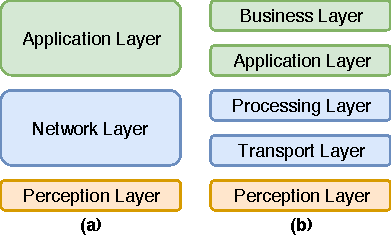
\includegraphics[scale=1.5]{Pictures/c2/2-2-IoT-architectures}
    \caption{Caption}
    \label{fig:2.3-iot-architecture}
\end{figure}


The three-layer architecture covers enough the main idea of the IoT, however, researchers often work toward the finer aspects of the IoT~\citep{Sethi:2017}.
Therefore, many more layered architecture were proposed to clarify the network layer and application of the three-layer architecture.
In the recent literature, the five-layer architecture~\citep{Wu:2010,Khan:2012} has been proposed with added \textit{transport layer}, \textit{processing layer} and \textit{business layer} as shown in Figure~\ref{fig:2.3-iot-architecture}b:
\begin{itemize}[noitemsep,nolistsep]
\item Transport layer: Differently from the network layer of the three-layer architecture, the transport layer only takes responsibility of transmission data from perception layer to the processing layer. It only includes networking technologies in this layer.

\item Processing layer: This layer is also known as middleware layer which is responsible for storing and processing data. Cloud computing and ubiquitous computing are the primary technologies in this layer.

\item Business layer: This layer manages the whole IoT system including applications, business and profits models. The success of the IoT not only depends on the advance of the updated technologies but also the innovation and reasonable of business model.

\end{itemize}

From system architecture perspective, the IoT systems can be classified into cloud-based systems and edge-based systems depending on where the processing layer take places.
In some architectures, for example, Cloud of Things~\citep{Jiehan:2013} or IoTCloud~\citep{Truong:2015}, data is processed in a large centralised fashion by cloud infrastructure.
On the other hand, in edge-based architecture, sensors, gateways, edge devices take part in data processing. 


\subsection{Cloud-based IoT Architecture}

%[Cloud infrastructure]
The widely accepted definition of cloud computing was phrased by the Nation Institute of Standard and Technologies(NIST)~\citep{Mell:2012} as 
‘‘Cloud computing is a model for enabling ubiquitous, convenient, on-demand network access to a shared pool of configurable computing resources (e.g., networks, servers, storage, applications, and services) that can be rapidly provisioned and released with minimal management effort or service provider interaction’’.
The cloud is composed of four layers: datacenter, infrastructure, platform, and application~\citep{Zhang:2010}.
Each of them can be seen as a service, for example, platform as a service (PaaS), infrastructure as a service(Iaas).
There are twofold benefits that the cloud computing can bring to the IoT: the virtually unlimited capability and resources~\citep{Zhang:2010}, and the scalable service delivery.

%[Cloud IoT Integration]
The integration of the could computing and the IoT was derived from the ideas that the cloud could be a bridge between IoT data collection, data processing, services delivering, filling the gaps of the lack of storage, computation and communication of IoT devices~\citep{Botta:2016}.
~\cite{Rao:2012} proved that the cloud can be an inexpensive and effective solution for things management from anywhere, at any time by using customised portals and built-in apps.
The huge amount of data produced by the IoT can be stored and processed by the datacenters which can on-demand storage capacity and processing capabilities that~\citep{Parwekar:2011}.
The ``everything as a service" paradigm of cloud computing can be applied on ``Things" introducing the ``\textit{Sensing as a Service}" paradigm~\citep{Zaslavsky:2013} or ``\textit{Things as a Service}" paradigm~\citep{Christophe:2011}.

\begin{figure}[ht!]
    \centering
    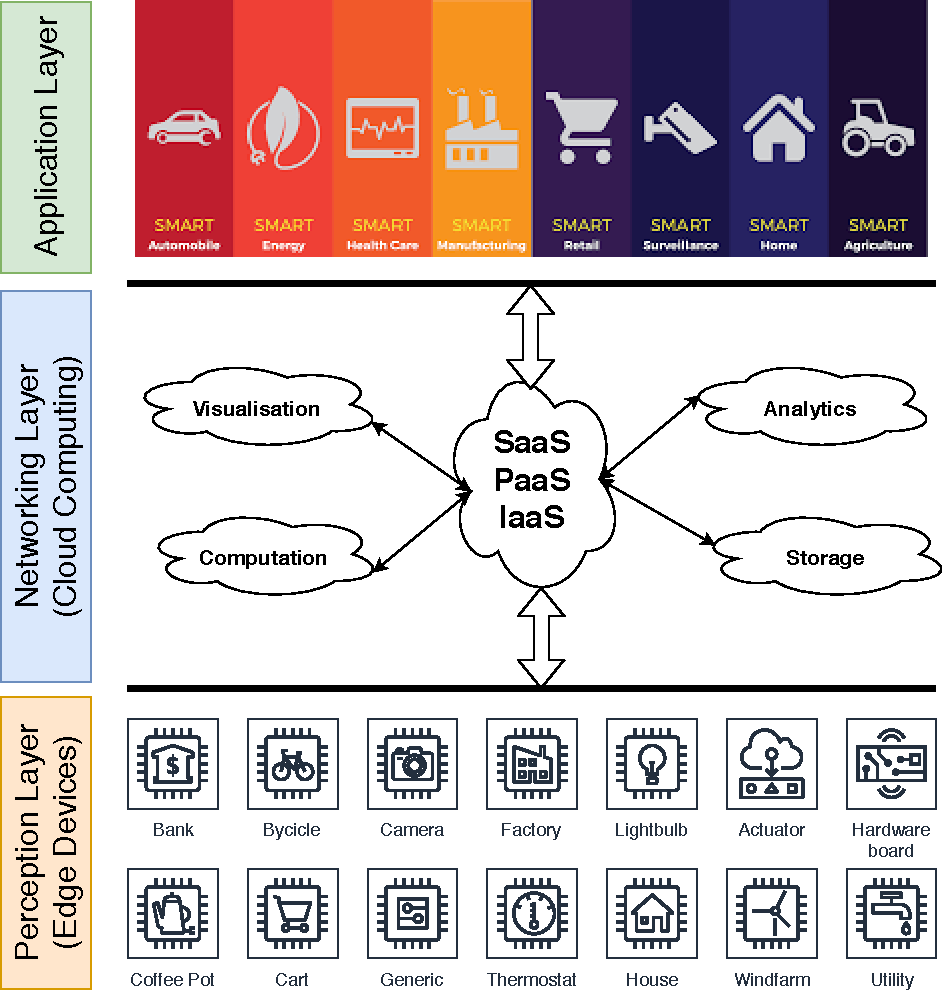
\includegraphics[scale=.65]{Pictures/c2/2-3-Cloud-based-architecture.pdf}
    \caption{Could based architecture}
    \label{fig:2.3.2-cloudIoT}
\end{figure}

Figure~\ref{fig:2.3.2-cloudIoT} illustrates an overview of architecture for the cloud of things. 
Data generated from the perception layer is sent through the communication layer to the cloud.
According to the requirements of the services, cloud provides storage and computation for data storing, data processing or data analysing. 
Once the service is created, it is made available from cloud for other applications to access.

There have been many 


\subsection{Fog/Edge-based IoT Architecture}

Although cloud infrastructures have been efficient for processing IoT data as computational resources on the cloud outclasses that of IoT devices at the edge, cloud-based IoT systems would encounter the issues related to network latency and traffic~\citep{Bonomi:2012,Zhang:2015,WShi:2016}.
The end devices in the IoT are not only data consumers as in cloud computing paradigm but data producers.
Therefore, the common approaches of directly connecting IoT devices and pushing IoT data to the cloud may have several disadvantages~\citep{Zhang:2015}.
The increasing of the number of the IoT devices means the quantity of produced IoT data is raising quickly.
Most of the data can be discarded immediately after being processed.
Hence, in these centralised systems, the bandwidth would be overwhelming and might be wasted.
Furthermore, pushing data into cloud will dominate upstream network traffic, meanwhile, broadband networks have more downstream bandwidth than upstream bandwidth.
Moreover, some IoT applications might require very quick response time, unfortunately, cloud-based solution may lead these applications to be less operable due to unexpected network latency.
In additional, IoT data might contain sensitive information from the sensors that are implanted surrounding us.
Cloud-based systems create more privacy and security concerns as centralised storage are out of users' control.
To address the issues of network overhead and network latency, and to improve the scalability for the IoT, the recent fog/edge based IoT architecture has been proposed~\citep{Bonomi:2014,Salman:2015}. 
As illustrated in Figure~\ref{fig:2.3.3-egdeIoT}, in fog/edge based system architecture, edge devices take part in data storing and data processing.

\begin{figure}[ht!]
    \centering
    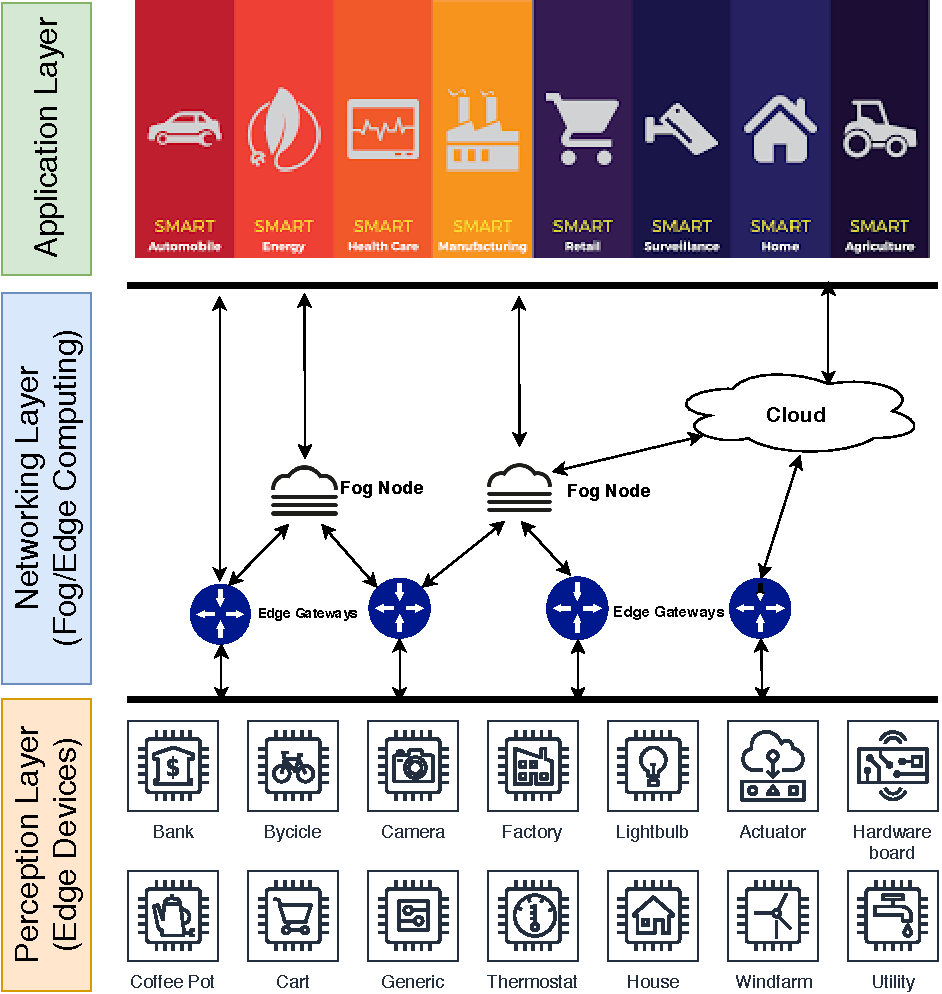
\includegraphics[scale=.65]{Pictures/c2/2-4-Edge-based-architecture.pdf}
    \caption{Caption}
    \label{fig:2.3.3-egdeIoT}
\end{figure}

\cite{Bonomi:2012} from Cisco stated that ``\textit{fog computing} is a highly virtualised platform that provides compute, storage and networking services between end devices and traditional Cloud computing Data Centres, typically, but not exclusively located at the edge of the network".
Meanwhile, \cite{WShi:2016} explained that ``\textit{edge computing} refers to the enabling technologies allowing computation to be performed at the edge of the network, on downstream data on behalf of cloud services and upstream data on behalf of IoT services".
Both fog computing and edge computing aim to provide the computation, storage, communication, services capabilities to the edge of network.

\cite{WShi:2016} defined the ``edge" as ``any computing and network resources along the path between data sources and cloud data centres".
In fog/edge based IoT architecture (see. Figure~\ref{fig:2.3.3-egdeIoT}),the fog/edge layer may include large number of edge/fog nodes which usually are routers, gateways, switchers, base stations or specific fog servers that are placed between end devices and cloud. 
Fog/edge nodes can be static at a fix point such as street light, house, offices or mobile on a moving objects such as smart phones or connected vehicle~\citep{Bonomi:2014}. 
These fog/edge nodes that have capabilities to compute, transmit and store the temporary data.
The end users can connect to these fog/edge nodes to obtain applications, services.
As fog layer is placed close to end users, edge/fog layer could support latency-sensitive applications, services.
Moreover, in the situation that more powerful computing and storage capabilities is required, fog/edge node can be connected to cloud. 



Both fog computing and edge computing paradigms is to decentralise and distribute data processing and storing from cloud to edge networks, these two terms are often used interchangeably.




For edge computing and fog computing, their architectures are hierarchical, decentralized, and distributed, which is different from centralized cloud computing architecture. 
Their service locations are the proximity to end users.
Edge computing is located in edge devices,while fog computing is located in network edge devices, which is single network hop or few network hops away from the edge. 
Their resources(e.g., computing, communication and storage resources) and computation and storage capabilities are limited by comparing with cloud computing, and edge computing is more limited than fog computing.
Because the resources and service capabilities of network edge devices are relatively stronger than edge devices. 
Moreover, these two computing paradigm have mobility support for end users. 
Because most services are provided locally, it is essential to take the existence of mobile devices into consideration. 
They also support the scalability of the whole ecosystem. 
The reason is that a large number of wide-spread and geo-distributed nodes are available if the situation requires them,including the nodes located at a certain site, neighboring nodes, or even the nodes situated at more remote geographical locations (Romanet al.,). 
Furthermore, they are highly virtualized computing platforms.
The nodes and networks are not always physical, while virtual sensor nodes and virtual sensor networks are also used for implementing various services (Aazam and Huh, 2014Aazam and Huh, 2014). 
The virtualized service mechanisms can be provided by them.

Obviously, even if they have the same goal, there are still some underlying differences between edge computing and fog computing. 
In edge computing, edge devices cannot implement multiple IoT applications, because the limited resources will result in resource contention and increase processing latency. 
While fog computing can overcome these limitations felicitously and avoid resource contention at the edge by seamlessly integrating edge devices and cloud resources. 
It coordinates the use of geographically distributed network edge devices and leverages the cloud resources to balance the use of resources and improve the utilization (Dastjerdi and Buyya, 2016). 
Furthermore,edge computing pays more attention to the things level, while fog computing focus more on the infrastructures level.

For edge computing and fog computing, their service locations are the proximity to end users. However, Edge computing is located in edgedevices, while fog computing is located in network edge devices, whichis single network hop or few network hops away from the edge. Edgecomputing platform usually tends to be constrained devices, whichbattery or storage capacities often are the limiting factors. When themultiple IoT applications need to be handled, this will result inresource contention and increases processing latency (Dastjerdi andBuyya, 2016). So the resource contention of edge computing is moreserious than fog computing. Moreover, edge computing focus more onthe things level, while fog computing focus more on the infrastructurelevel


\begin{table}[ht!]
    \centering
    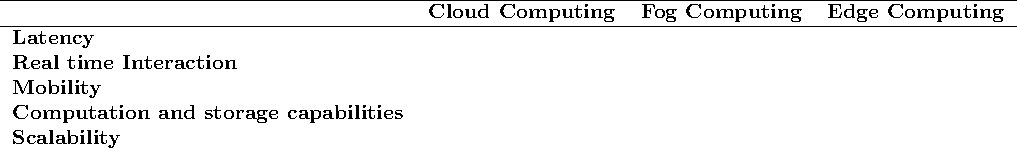
\includegraphics[scale=.75]{Table/2-3-edge-fog-cloud.pdf}
    \caption{Caption}
    \label{tab:my_label}
\end{table}

The edge computing has been emergent and benefit for the IoT~\citep{Yu:2018}. 
There have been several early results that demonstrated the benefit of applying edge computing. 
Face recognition application could run 4 times faster by moving computation from cloud to edge~\citep{Yi:2015}.
Using cloudets for offloading computing tasks did not only reduce the response time for wearable cognitive assistant but also save 30$\%$ to 40$\%$ energy consumption~\citep{Ha:2014}. 
However, computing nodes often have less computational resource and networking capability. 
This poses a challenge for the computing tasks to be physically moved to the edge nodes.



\section{Summary}

IoT developments during recent years have been characterized by
attributes that can be “labelled” the 6As: Anything (any device), to be
transferred from/to Anyone (anybody), located Any place (anywhere), at
Any time (any context), using the most appropriate physical path from Any
path (any network) available between the sender and the recipient based
on performance and/or economic considerations, to provide Any service
(any business). The IoT paradigm is evolving and entire IoT ecosystems
are now built upon innervation elements known as the 6Cs: Collect (het-
erogeneity of devices of various complexities and intelligence, that enhance
the real-time collection of data generated from the connections of devices
and information), Connect (ubiquitous distributed connections of heteroge-
neous devices and information, where the connections are the foundational
component of the IoT), Cache (stored information in the distributed IoT com-
puting/processing environment), Compute (advanced processing and com-
putation of data and information), Cognize (information analytics, insights,
extractions, real-time AI processing and Create (the creation of new interac-
tions, services, experiences, business models and solutions). This is illustrated
in Figure 3.1






















\nop{

%==================================================================================================
\section{The Semantic Web technology}
\label{s:sw}
%==================================================================================================

According to World Wide Web Consortium(W3C), the Semantic Web technologies aim to ``provide a common framework that allows data to be shared and reused across application, enterprise, and community boundaries".
The Semantic Web community has developed a suite of standards and technologies to formally describe the semantics, support automated reasoning on web data.
As we mentioned in Section~\ref{ss:stiot}, such technologies developed by the Semantic Web are potentially the solutions to data integration, semantic interoperability, context awareness and knowledge transformation in the IoT.
This section introduces the core technologies of the Semantic Web that including Resource Description Framework~\citep{Lassila:1999},RDF schema~\citep{Dan:2004}, Web ontology language~\citep{Guinnes:2004} and SPARQL query language~\citep{Eric:2008}.

%===================================================
\subsection{RDF Data Model}
\label{ss:rdf}
%===================================================
A \textit{data model} is an abstraction that is used to represent the information of real world entities.
It defines how the properties and relations of the entities are represented, and the operations can be performed on the information.
Data models can be categorised as relational, tree and graph based. 

\begin{figure}[ht!]
	\centering
	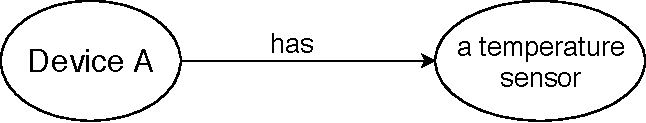
\includegraphics[scale=.65]{c2/2-2-SimpleTriple.pdf}
	\caption{A triple}
	\label{fig:2.2-simpleTriple}
\end{figure}

RDF data model is a graph-based data model. 
Its design is based on the idea that things can be represented by statements in a simple manner of triples. 
The statement is similar to a simple sentence that has subject, verb, object.
The triple is composed of three elements: a subject, a predicate and an object that represent the statement.
For example, the sentence "Device A has a temperature sensor" can be expressed as a triple as follows: ``Device A" is the subject, ``has" is the predicate and ``a temperature sensor" is the object.
The statement can be visually expressed in Figure~\ref{fig:2.2-simpleTriple}

An RDF triple is built from \textit{IRIs} (International Resource Identifiers), \textit{literals} and \textit{blank nodes} which are also called \textit{resources}~\citep{Cyganiak:2014}. 
RDF triple can be formally define as follow:
``An RDF triple is a tuple (S, P, O) $\in$ (I$\cup$B)  $\times$ I $\times$ (I$\cup$B$\cup$L), where S is the subject, P is the predicate and O  is the object and I, B and L are used to represent IRIs, blank nodes and literals respectively."

The IRI is a unique identifier that presents a thing or a concept.
For example, the IRI for representing the device A in the previous example might be ``\textit{http://insight.org/device/A}". 
The IRI ``\textit{http://insight.org/sensor/temperature}" can refer to the concept of ``temperature sensor".
Literals are used to represent value data types such as numbers, booleans or strings. 
A literal might be a simple string such as ``a temperature sensor", or with a optional language tag, ``a temperature sensor"$@$en, 
denoting the language (English), or with an IRI, ``temperature sensor"{\symbol{94}\symbol{94}}\textit{http://www.3.org/2001/XMLSchmea$\#$String}, assigning the datatype (String). 
The blank node (B-Node) is used to refer to a concept with giving it a name. 
The usage of the blank will be explained shortly in the later example.

In an RDF triple, the subject is an IRI or a blank node as it must refer to a concept. 
The object can be an IRI, a blank node or literal. 
The predicate is guaranteed to be an IRI denoting a bi-relationship between the two resources. 
Figure~\ref{fig:2.3-SimpleRDFTriple} shows the presentation of the previous example statement as an RDF triple.

\begin{figure}[ht!]
	\centering
	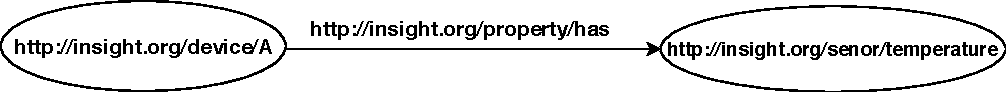
\includegraphics[scale=0.75]{c2/2-3-SimpleRDFTriple.pdf}
	\caption{An RDF Triple }
	\label{fig:2.3-SimpleRDFTriple}
\end{figure}

An RDF document is a set of RDF triples.
The RDF document can be represented as a directed graph as illustrated in Figure~\ref{fig:2.4-SimpleRDFGraph}.
The nodes represent subjects and objects, the predicates are represented by labelled edges with the direction from subjects to objects. 
Therefore, RDF documents are also called RDF graphs.

\begin{figure}[ht!]
	\centering
	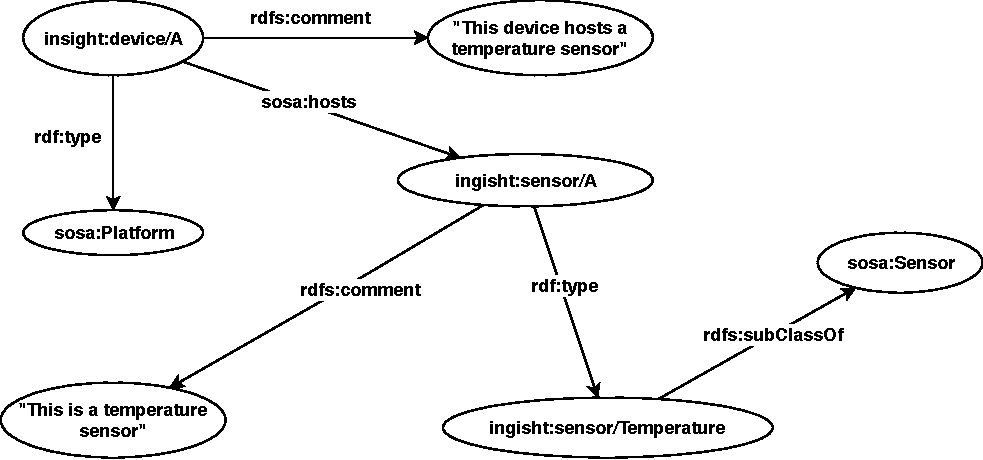
\includegraphics[scale=0.65]{c2/2-4-SimpleRDFGraph.pdf}
	\caption{RDF document describing device A as an RDF Graph.}
	\label{fig:2.4-SimpleRDFGraph}
\end{figure}

\textit{Vocabularies} are used to define concepts and their relations that related to a specific domains. 
For example, to describe people and their relationship, FOAF~\citep{Dan:2010} can be used.
SSN~\citep{Armin:2017} is another RDF vocabulary used for describing devices, sensors.
An RDF vocabulary is a collection of IRIs that used for describing schema and instance data.
The IRIs in an RDF vocabulary are often created with a common substring in the beginning which is called \textit{namespace} of an vocabulary.
For convenience, prefixes can be used to shorten the string representation of these IRIs.
Figure~\ref{fig:2.4-SimpleRDFGraph} illustrated the RDF document describing the devices A from the previous example.
RDFS vocabulary~\citep{Dan:2014}, which is used to defined and documented additional RDF vocabularies, and the SSN vocabulary are used.
For simplicity, prefixes are use the replace the namespaces and the list of prefixes and their corresponding namespace is shown in Listing~\ref{lst:prefixes}.

\vspace{5mm}
\begin{lstlisting}[language=sparql,
  				   captionpos=b,
                   label={lst:prefixes},
                   caption={Prefixes}]  
rdf  : <http://www.w3.org/1999/02/22-rdf-syntax-ns#>
rdfs : <http://www.w3.org/2000/01/rdf-schema#>
sosa : <http://www.w3.org/ns/sosa/>
geo  : <http://www.w3.org/2003/01/geo/wgs84_pos#>
insight : <http://insight.org/>
\end{lstlisting}


The flexible and expressivity of triple lead RDF data model become a great ideal to deal with the dynamic and heterogeneity of the IoT.
RDF  provides both ability to specify concept and ability to link different concepts together.
This enables heterogeneous IoT data to be update and integrated with extremely low effort.

\begin{figure}[ht!]
	\centering
	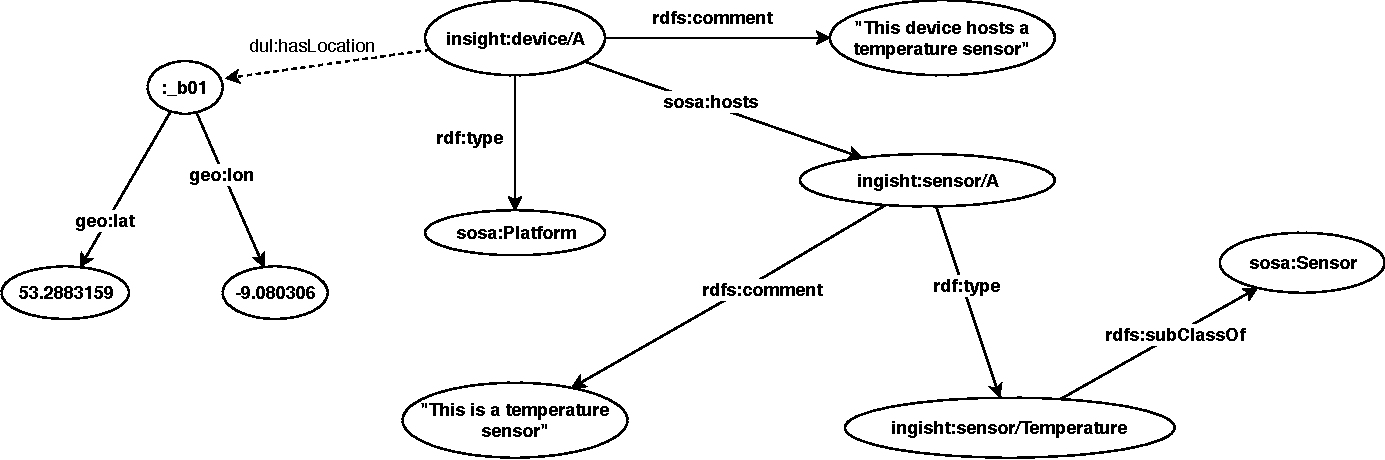
\includegraphics[scale=0.65]{c2/2-5-RDF-integration.pdf}
	\caption{Example of integration RDF graph describe device and RDF graph describing geographic coordinates}
	\label{fig:2.5-integration}
\end{figure}

As a graph data model, to represent information, RDF does not require a predefined data schema as relational databases does.
New type of information, new concept can be introduced without the need of updating data schema.
For example, to give the device A a location requires an integration of the RDF graph from Figure~\ref{fig:2.4-SimpleRDFGraph} with another RDF graph that describes the geographic coordinates.
In Figure~\ref{fig:2.5-integration}, the latitude and longitude values can be added to the RDF graph without introducing what are they.
The machine can understand via the vocabulary that is used to describe the values.
The integration is done by adding a triple to say that device A has located at a point which has the latitude, longitude values as in the figure.
This is much easier than realigning the data schema in case using common relational data model. 
In this example, the location is presented as a blank node as it does not have to be an IRI.

RDF data model allows data to be reusable and shareable.
The same vocabularies can be used in different applications, systems from different domains to describe the same thing.
For example, the vocabulary describing coordinates in a geographic application can be used to describe the location of the device.
Further more, with inferencing (see Section~\ref{ss:inference}), new relationships or concepts can be discovered from the the base relationship found in dataset.
This helps machine to determine if different vocabularies were used to describe the same concept.
In the previous example, the sensor ``\textit{insight:sensor/A}" is defined as ``\textit{a temperature sensor}" using IRI ``\textit{insight:sensor/Temperature}".
By defining ``\textit{insight:sensor/Temperature}" is the subclass of ``\textit{sosa:Sensor}", machine can understand that ``\textit{insight:sensor/A}" also refers to a sensor.
Thus, ``\textit{insight:sensor/A}" is understandable and discoverable as a sensor by another systems or applications that are using SSN vocabulary.

\textit{Linked Data} is an approach for publishing and consuming structured data on the Web using RDF data model.
The principles of Linked data include: (i) Using URIs for naming things; (ii) Using HTTP URIs to enable the look up on things; (iii) Describing the information of the URIs using RDF data; (iv) Including the links to other URIs, so that they can discover more things. 
The same principles can be applied for publishing and consuming IoT data, for example, sensor data~\citep{Patni:2010} or stream data~\citep{Sequeda:2009}.
Linked Data can make data linkable and discoverable thus becomes an efficient solution for the fragmentation issue in the IoT.
RDF data model provides a flexible way to describe things and their relationship, such as devices, observations or measurements. 
RDF vocabularies and inference allow semantics, knowledge to be shared crossing devices, systems and platforms. 
Using Linked Data principles and RDF data model could enable the semantic interoperability for the IoT in the global scale~\citep{Le-Phuoc:2018}.

%===================================================
\subsection{Inference}
\label{ss:inference}
%===================================================

As we mentioned in the previous example, the Semantic Web technologies do not only provide RDF data model to describe concepts and theirs relationships but also the ability to discover new relationships from the given dataset.
This ability is known as inference.
\textit{RDFS}(RDF schema)~\citep{Dan:2004} and \textit{OWL}(Ontology Web Language)~\citep{Guinnes:2004} are the two standards to create vocabularies that enables the inference.

RDFS is derived from RDF by adding some basic constructs to allow the inferencing on the type of things and properties of things.
RDFS is added classes and subclasses to specify different concepts and to describe if two concepts are related.
As shown in the example (see Figure~\ref{fig:2.5-integration}), the device and the sensor are differentiated by the class ``\textit{sosa:Platform}" and ``\textit{insight:sensor/Temperature}". 
The additional triple that says the type ``\textit{insight:sensor/ Temperature}" is a subclass of the type ``\textit{sosa:Sesnor}" infers that the sensor also has type ``\textit{sosa:Sesnor}".
The further additional features are property domains and ranges.
The domains of a property state that any subject that has this property is an instance of a specific class or set of classes.
The ranges of a property define the specific classes (types) that its object can be.

OWL provides more inferencing capability. 
OWL enables the ability to share not just information, but vocabulary.
For example, OWL includes ``\textit{owl:sameAs}" to state if two classes or two properties are the same.
With OWL supporting, two systems that do not use the same vocabulary to publish RDF data might be able to understand and process data the other. 

%===================================================
\subsection{SPARQL Query}
\label{ss:sparql}
%===================================================

SPARQL has been standardised as the query language query RDF data by the the World Wide Web Consortium~\citep{Eric:2008}.
To query graph-based data, SPARQL is designed as a graph-matching query language.
The graph pattern in a SPARQL query can be simple with a single triple pattern of very complex.
Given an RDF graph G and a query Q that consists of a graph pattern, the values obtained form the matching of the pattern against G are formed the answer.

A triple pattern is similar to an RDF triple in which subject, predicate, object could be a variable.
A set of triple pattern forms a basic graph pattern. 
Listing~\ref{lst:SPARQL1} is showing Q1, an example of a SPARQL SELECT query with a simple graph pattern containing a triple pattern.
The query asks for the list of the sub-systems that are hosted on the Device A.

\vspace{5mm}
\begin{lstlisting}[language=sparql,
  				   captionpos=b,
                   label={lst:SPARQL1},
                   caption={Q1 - SPARQL Query with a graph pattern}]  
PREFIX sosa    : <http://www.w3.org/ns/sosa/>
PREFIX insight : <http://ingisht.org/>

SELECT ?subSystem WHERE
{ 
  <insight:Devcie/A> sosa:hosts ?subSystem.
}    		
\end{lstlisting}


A basic graph pattern matches against a RDF graph when the variables can be replaced by values from the graph and form a subgraph of the graph.
For example, the IRI ``\textit{insight:sensor/A}" is replaced the variable ``\textit{?subSystem}" to form a subgraph of the RDF graph in Figure~\ref{fig:2.4-SimpleRDFGraph}.
This value is the answer of the query Q1 against RDF graph in Figure~\ref{fig:2.4-SimpleRDFGraph}.

A more complex may contains more than one basic graph pattern.
A resultant RDF subgraph can be further queried or joined with the results of other basic graph patterns to answer the query.
The query Q2 in Listing~\ref{lst:SPARQL2} asks for a list of subsystems on the device A that are temperature sensors.
The query contains two basic graph patterns, the first pattern asks for the subsystem on the device A and the second pattern asks if its is a temperature sensor.

\vspace{5mm}
\begin{lstlisting} [language=sparql,
  				   captionpos=b,
                   label={lst:SPARQL2},
                   caption={Q2 - SPARQL Query with multiple graph patterns}]                    
PREFIX ssn  : <http://www.w3.org/ns/ssn/>
PREFIX ex   : <http://example.org/>
PREFIX rdf  : <http://www.w3.org/1999/02/22-rdf-syntax-ns#>

SELECT ?subsystem WHERE
{ 
  <insight:Devcie/A> sosa:hosts ?subSystem.
  ?subSystem rdf:type <insight:sensor/Temperature>
}    		
\end{lstlisting}

SPARQL queries may also have additional operations including unions, optional, filter, subqueries, value aggregations, path expressions, etc.
The examples of SPARQL queries with other operations can be found in Appendix~\ref{app:A}.
Formally, a SPARQL graph pattern is a basic graph with or without these additional operations and can be summarised as following:
\begin{itemize}[noitemsep,nolistsep]
\item \textit{Group graph patterns:} A set of graph patterns delimited by braces $\{$ $\}$.
\item \textit{OPTIONAL patterns:} A graph patten identified by OPTIONAL keyword to mark this graph pattern as an optional graph pattern. 
                                  This means, the result set is returned even if the variables in the optional graph pattern are not bound.
\item \textit{UNION patterns:} Keyword UNION is used to combine graph patterns with alternative graph patterns that may match.
\item \textit{FILTER expressiond:} FILTER is used to eliminated the solution that is not match specific conditions. 
                                   The filter may be a comparison expression, logical connectives or built-in function.
\item \textit{Subqueries:} Embedded SPARQL queries that are nested inside a SPARQL query to limit the result set.
\item \textit{Property paths:} Property path is used to define the possible route through an RDF graph between two RDF nodes. 
\end{itemize}

\cite{Perez:2009} defined a SPARQL graph pattern recursively as following:
\begin{enumerate}[noitemsep,nolistsep]
\item A triple pattern is a graph pattern.
\item A graph pattern is a graph pattern.
\item If P$_{1}$, P$_{2}$ are graph pattern, then (P$_{1}$ AND P$_{2}$), (P$_{1}$ OPTIONAL P$_{2}$) and (P$_{1}$ UNION P$_{2}$) are graph patterns. 
\item If P is a graph pattern and F is a FILTER expression, then (P FILTER F) is a graph pattern.
\item If P is a graph pattern and G $\in$ ($U \cup V$), then (GRAPH G P) is a graph pattern.
\end{enumerate}

\cite{Perez:2009} also proved that for a given RDF data D, a graph pattern P, to evaluate if a mapping $\mu$ is the a result of matching 
P against D, the complexity can be summarised as follow:
\begin{itemize}[noitemsep,nolistsep]
\item The evaluation can be solved in time \textbf{O($|$P$|$.$|$D$|$)} for graph pattern expressions constructed by using only AND and FILTER operators.
\item The evaluation is \textbf{NP-complete} for graph pattern expressions constructed by using only AND, FILTER and UNION operators.
\item The evaluation is . Evaluation is \textbf{PSPACE-complete} for graph pattern expressions.
\item The evaluation(P) is in \textbf{{LOGSPACE}} for every graph pattern expression P.
\end{itemize}

In practice, SPARQL processors often join the triples that match triple patterns in a basic graph pattern. 
A basic graph pattern can be formed as a directed graph and it has different shapes(see. Figure~\ref{fig:2.6-bgp}). 
The shape of the graph pattern also defines the complexity of the matching, because, each shape requires a specific joining plan~\citep{Hartig:2014}.
The shapes of a basic graph pattern are: 
\begin{itemize}[noitemsep,nolistsep]
\item \textit{Chain} shape contains of object-subject joins as triple patterns are connected like a chain.
\item \textit{Star} shape contains subject-subject joins as the join variables are the subjects of the triple patterns.
\item \textit{Snowflake} shape is a combination of star shape and chain shape.
\end{itemize}

\begin{figure}[ht!]
	\centering
	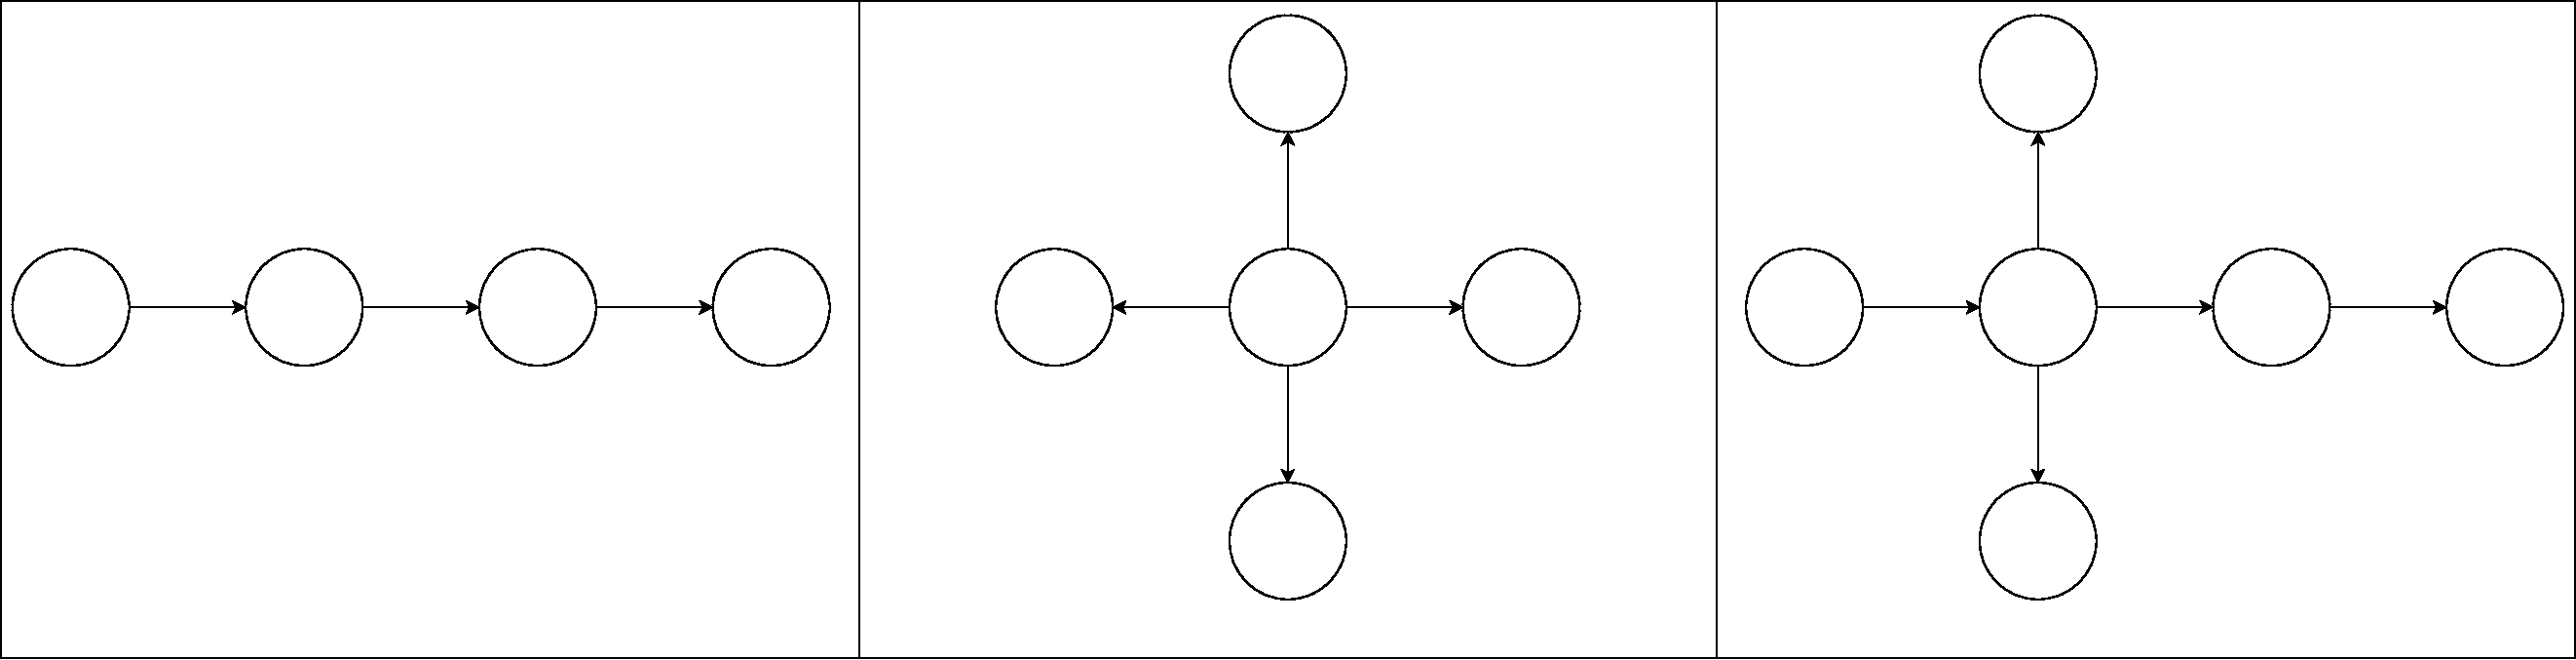
\includegraphics[scale=0.25]{c2/2-6-BGP-shape.pdf}
	\caption{Shape of basic graph pattern: chain, start, snowflake from left to right respectively.}
	\label{fig:2.6-bgp}
\end{figure}

SPARQL also supports other types of query apart from the SELECT query that was shown in the previous example. 
\begin{itemize}[noitemsep,nolistsep]
\item \textit{ASK} query to pose a ``yes/no" query and retrieve a binary ``true/fasle" in return.
\item \textit{CONSTRUCT} query to create new RDF graphs from a query return.
\item \textit{DESCRIBE} query to return details information of a resource.
\end{itemize}

Since the RDF data model allows heterogeneous data to be semantically described and linked, the SPARQL allows the data to be semantically extracted, integrated.
With the ability of expressing semantic search criteria, SPAQL could be the semantic query language for discovery heterogeneous things in the IoT~\citep{Richard:2013,Chun:2015}.
The newer version, SPARQL 1.1~\citep{Harris:2013} has included update and federation that is more adaptable to the dynamic and distributed environment of the IoT. 
C-SPARQL~\citep{Barbieri:2009} and CQELS~\citep{Le-Phuoc:2011} are the two query languages that extend SPARQL to enable evaluating linked stream data.


\section{Storing and Querying RDF data}
\label{s:sq}

In the previous section, we presented the overview of RDF data model and SPARQL.
This section provides an overview of how RDF data is stored and SPARQL query is executed. 
This topic is definitely important.
Understanding how RDF data is processed could help the later decisions on selecting data structures and algorithms.
Every data structures and algorithms have their own advantages and disadvantages in different situations.

\subsection{Physical organisation for RDF data}

The basic schema of RDF storage can be constructed simply.
For example, \cite{Harris:2005} represented RDF using relational model and SPARQL queries can be answered by translating to SQL queries.
The approach was demonstrated with 3Store that runs of MySQL, a relational database.
3Store uses a single table to store RDF graph and each triple is stored in a row. 
Each field in the triple table stores a hash value and the actual string values are stored in a symbol table, keyed on the hash value.
A constraint of this model is not only the translation of SPARQL queries to SQL queries, additional SQL queries might be required to determine the string representation from the returned hash values. 
3Store simplified the additional search constraint by joining the hash values back onto the triple table.

The approach of building RDF store using a back-end relational database was common in the Semantic Web community. 
Redland~\citep{Beckett:2001}, Sesame~\citep{Broekstra:2002}, Jena~\citep{Wilkinson:2003} and Virtuoso~\citep{Erling:2009} were the notable systems of this kind of RDF store.
This approach is quite simple and flexible, RDF graph can be stored in a generic fashion without a need of any customisation.
However, real relational DBMSs do not seem to be suitable to store RDF data in this fashion.
These systems rely on the optimisers of the back-end databases to optimise the queries.
This makes challenging for the databases to collect or produce relevant information for the optimisation.
The triple tables are exceptionally long and thin (little information per row). 
Useful amount of information requires a lot of rows to store.
Searching for a piece information becomes more difficulty since the number of rows increases.
Because, to return a query, the triple table has to be joined to itself and a query involves lots of joins rapidly becomes costly.

\cite{Abadi:2007} proposed to store RDF triples in different table called Property Tables.
Each table was assigned to a property and stored only the subject and object that are connected by the property. 
Despite the substantial advantages showed in the initial results of this proposal, a later evaluation showed that the performance improvement could be reduced if using different sort order  for the triple table approach~\citep{Schmidt:2008}.

RDF triples typically are stored in one or few long triple tables, iterating through the whole table to find one or some particular triples is impractical. 
Indexing can provide shortcuts to specific pieces information that a query requires. 
If indexes are available on one or several attributes, the search can jump straight to the triples that contain the search values.
The modern RDF stores create their own indexing strategy to index triples and overcome their large triple tables handicap.
Many stores, such as Hexastore~\citep{Weiss:2008} or RDF-3X~\citep{Neumann:2010}, do not need to store triples in table, because their indexes cover all possible access patterns.

The the idea of creating index for RDF graph is to allow efficiently retrieving the RDF triples that match a triple pattern. 
For example, the RDF triples that match the triple pattern (S P ?) can be retrieved on SPO index, in which S and P are keyed (S stands for subject, P for predicate and O for object).
The indexes are created materialising all possible of orders that cover all triple patterns.
Using three combinations of nodes in a cyclic ordering is enough to cover all query patterns (SPO, POS, OSP).
However, some RDF stores create less or more indexes depending on their query optimising or executing strategy.
Particularly, Hexstore and RDF-3X employ six index permutations, allowing them use merge joins that fastens the query executing.
Furthermore, the indexes contain all the data, so all the work can be done within them.

Selecting data structure to maintain these indexes is specially important for RDF storage.
Storing RDF triples in an optimal manner, such as multiple indexes, gives the accesses to matching triples more efficient.
Searching for the matched triples still slow if it requires to scan the whole index.
Data structure does not only influence the efficiency of searching but inserting, updating and the compactness of the storage.

There are variety of data structures, each of them is suitable for different tasks. 
Hash table or hash map are the data structures that are commonly used for memory-based storage~\citep{Date:1990}.
The part of the data that is as key search is hashed. 
A pointer to the location of the data in the database is stored at the memory position corresponding to the hashed value.
Hash data structure offers good performance as inserting and searching on hash table are $O(1)$ time complexity operations.
Popular RDF stores, such as Sesame~\citep{Wilkinson:2003}, SwiftOlwim~\citep{Ognyanoff:2007} and Jena~\citep{Seaborne:2010} used hash table to store RDF graph in memory.

However, some characteristics of hash data structure make it less desirable for disk-based RDF storage.
Of course, suitable hashing algorithm has to be utilised, otherwise, many hash collisions may occur.
In the point of view of SPARQL, to retrieve the set of triples that match a triple patterns, range searches are often utilised.
Meanwhile, hash does not provide physically ordered data based on its logical order, for example sorted order. 
That means it does not guarantee if two entities that are similar to each other are stored next to each other.
Triples that match a triple pattern are not guarantee to be stored in a same disk block or a sequence disk blocks.
Disk seek would be required for retrieving every single triple, creating massive searching and reading.

B-tree data structures, in particularly the B$^+$-tree variants, are the most common data structure for implementing disk-based indexes~\citep{Comer:1979}.
B-tree data structures are self-balance tree structures.
Each node in a B-tree has a number of child nodes.
The height of a tree is proportionate to log$_{n}$ where n is the fanout - the number of child nodes that a node can have.
The size of the fanout defines the height of a tree, and the height of the tree equals to number disk seeks required to search a data item. 
The height of the tree can be reduced by increasing the size of the fanout.
Consequently, the number of comparisons required to determine the child nodes to access increases when the fanout gets larger.
B-tree data structure is useful for hard disks because they can make a good use of such block-based memory medium's characteristics by keeping the tree nodes sized to a block.
A disk block (typically around 4kB-8kB) is quite large, hence, the height of the tree is often low, of course, few disk seeks are required. 
Retrieving a block costs equally to retrieve partial block.

B$^{+}$-tree is a variant of B-tree that modifies B-Tree.
B$^{+}$-tree allows all pointers to actual data to be stored in the leaf nodes, and leaf nodes are linked to allow sequential traversal over them.
Comparing to hash data structure, B-tree offers much better performance for range search~\citep{Ullman:2001}.
Therefore, B$^{+}$-tree has been attracted to creating indexes for RDF data.
The relational databases that have been used as back-end database for RDF triple store made exclusive of this data structure. 
The other systems, such as Jena TDB~\citep{Owens:2008} or RDF-3X~\citep{Neumann:2010}, were implemented with their own versions of B$^{+}$-tree.

The approaches seem to be attractive to store RDF data for cloud-based system or IoT nodes that are powerful workstation.
Processing RDF data on the edge nodes would be more challenging.
The environment on the edge IoT is more dynamic, hence updating ability is more important.
Using memory-based RDF storage using hash table could be a suitable solution as inserting with hash table is O(1) time complexity operation.
However, IoT edge nodes often have limited memory, memory-based storage would not scale on edge nodes. 
Disk-based storage would enable more data can be stored on edge nodes.
However, edge nodes are often equipped with flash-based storage.
B-tree data structure is not well-suited with the characteristics of this type memory medium.


\subsection{SPARQL Processing}

A SPARQL query is often processed in the followings sequential step:
\begin{enumerate}[noitemsep,nolistsep,label=(\roman*)]
\item Compile SPARQL query to an internal form and convert it to canonical form;
\item Choose the candidate physical operators;
\item Generate the query plans and choose the cheapest on to execute. 
\end{enumerate}

The first step transforms the query string to an internal format that is easier to process further. 
In this step, some minor optimisations can be utilised such as removing irrelevant triple patterns.
The second step is to produce low-level operations for processing the query for example, index scanning or joining.
The operations are selected associatively with the information, such as data structure on disk, availability of indexes or statistic of data, to speed up the query. 
In this step, the cost of executing of each operation is calculated and is assigned to them.
In the final step, a set of potential query plans are created from the operations produced from the previous step. 
In a query plan, the operations and the order in which the operations are performed influence the performance of a query.
Choosing the best query plan is also performed in this step. 
A cost model is assigned to compute cost for each query plan.
The cost model is often based on the selected operations and the order in which the operations will be performed.
The cheapest query plan will be chosen and executed.

Answering a SPARQL query requires multiple joins of RDF triples that match the triple patterns.
This leads join operation to be the most-used while executing SPARQL queries. 
Different join algorithms are differentiated by how the input data is organised and require different amount of computing resource to perform.
Indexed nested loop, hash join and sort/merge join are the join algorithms that are useful for joining RDF data~\citep{Owens:2011}.

The index nested loop join~\citep{DeWitt:1993}(INLJ) uses nested loop to for joining two sets. 
For each item in one set (called the outer input), it scans the entire the other set(called the inner input) and finds compatible items.
The performance of INLJ relies on the availability of index on the inputs.
This algorithm is faster than the brute force algorithms which often have O(n$^{2}$) time complexity with n is the size of the data being examined.
If index is available on the inner input and there is no match, only few operations need to be utilised in stead of scanning entire inner set.
This algorithm is especially effective in terms of reducing computation in the situation that:
the outer input is small and the inner input is very large.
INLJ is useful for utilising join over RDF data since RDF stores are often designed with comprehensive indexing strategies~\citep{Owens:2011}.

Hash join is the algorithm for joining two set based on hash function~\citep{Ullman:2001}. 
It performs two single scans over the inputs.
The first scan is to create hash table for the first input.
The hash table contains hashed value of join attributes of each item and a corresponding pointer to the item. 
The compatible items on the second input are found by scanning and looking back to hash table.
This algorithm does not require indexing on inputs and scales in a linear manner with the size of the inputs.

Merge join algorithm requires the items in two input set are sorted on the join attributes~\citep{Ullman:2001}.
Therefore, the join can be execute by simply scanning of both inputs and comparing on the join attributes to produce join results. 
Sort/Merge join simply sorts the inputs as required and performs merging.
Merge join is always faster than hash join or nested loop join if data is sorted correctly.
However, in case the inputs have to be sorted, the performance of this algorithm largely relies on the performance of the sorts.

Selecting the right algorithms for implementing the join operations of query processors is obviously important.
Especially, many join operations may be required to execute SPARQL query, and they contribute the most on time consumption and resource consumption of SPARQL processing. 
The INLJ join requires very little memory and also is efficiently for paralleling~\citep{Sheu:1991}.
However, in disk-based stores, INLJ might require higher number of disk seeks comparing to hash join or sort/merge joins.
Hash join does not require searching or sorting as data can be scanned sequentially on disk, but memory is required to hold the the intermediated results.
It is less tractable if no memory is available.
Merge join is fastest algorithm if sorting is not required. 
For this reason, RDF engines such as, RDF-3X~\citep{Neumann:2010}, often try to use merge join as possible. 
RDF-3X orders the join operations accordingly to the sort order of data in the working set.

Selecting the right joins is more challenging to execute SPARQL on IoT edge nodes.
The former query planners and query optimisations select the joins and order the joins with out taking resource consumption(memory consumption) into account. 
Of course, in unlimited capabilities storage and processing power environments such as cloud infrastructure, minimising the time spend on the join is the highest priority. 
On the edge nodes, resource consumption of the joins must be considered as inappropriate resource usage may result system failure.

\section{Summary}

In this chapter, the relevant concepts in the IoT, the Semantic Web and the fundamental RDF data processing was introduced as the research background of the thesis.
Section~\ref{s:iot} introduces three visions of the IoT: Thing-oriented vision, Internet-oriented vision and Semantic-oriented vision.
This section also highlights the need of the semantic technologies in solving the interoperability problems and the emergence of the edge computing for the IoT. 
In section~\ref{s:sw}, the suite of Semantic Web technologies including RDF data model, inference, SPARQL query language are introduced.
RDF data model is a graph-based data model which allows a flexible way to describe things properties, things relations and link different things together.
The inference ability allows RDF data to be reasoned to derive new concepts, new relations from a base dataset, therefore, allowing the meaning of data to be shared.
To query RDF data, SPARQL query language was designed as graph-matching query language.
SPARQL allows the data to be semantically extracted, integrated.
How RDF data is stored and SPARQL query is executed is presented in Section~\ref{s:sq}.
Indexing is critical important for the RDF data to be stored to allow efficient querying.
Storing RDF in-memory will allow fast inserting and querying, however, memory on the edge nodes is usually not enough to hold all the data in the memory. 
B-tree is most common data structure to implement indexes for RDF data in disk-based RDF storage.
However, B-tree may not suitable for flash-based storage and this issue will be more precisely presented in the next chapter.
Answering SPARQL query requires many join operations to be utilised.
Different algorithms for implementing joins result different time consumption and resource consumption of joins.
Executing SPARQL query on IoT edge nodes requires the query planners and optimisers take resource consumption into account.
}









